%*****************************************
\chapter{3D Spieleentwicklung mit Java}\label{ch:beispiele}
%*****************************************

\section{Allgemeiner Aufbau von 3D Spielen}\label{sec:aufbau}
Hier erklären wir, wie 3D Spiele funktionieren, worauf es ankommt, welche Möglichkeiten/Schwierigkeiten man hat und so weiter. (Vector3f...)

\section{Funktionsweise der jMonkeyEngine}\label{sec:jMonkeyEngine}
Erklärung wie wir auf die Engine gestoßen sind, welche anderen engines es gibt und was die Vorteile der Engine sind. Vielleicht auch Hinweis dass die doku inzwischen veraltet ist usw...

\section{Umsetzung in Programmcode}\label{sec:code}
Erklärung wie man verschiedenste Funktionalitäten in jme3 umsetzt.

\subsection{Erzeugung der Application-Klasse: SimpleApplication}
Allgemeine Erklärung welche Klassen verwendet werden und wie man eigentlich ein spiel aufbaut. Auch hinweis auf die 3 Methoden in der Klasse und was diese machen

\subsection{Funktionsweise von Nodes}
Erklären, dass es verschiedene Nodes z.B. Gui/Root... usw gibt und entsprechende Elemente dort attached werden können.
Vorteil: Es können alle Kinder einer Node gleichzeitig angesproechen werden. Baumstruktur...

\subsection{Modelle}
Hier könnte noch die Animation erwähnt werden, welche in unserem Spiel nicht genauer berücksichtigt wird.
Auch mit rein bringen was modelle eigentlich sind und wie man welche erstellt, sowie Datentypen (jme3 Objekt, obj, 3ds,, und was es alles gibt)
\begin{itemize}
	\item Wie werden sie erstellt
	\item Wie lässt man sie bewegen
	\item Siehe Tutorial...
\end{itemize}

\subsection{Materialien}
Erklärung der Materialien und wie diese über z.B. Blender oder intern verwendet werden können.
Beispielbild wie ein Element mit / ohne Material aussieht.

\subsection{User-Input}
Welche möglichkeiten zur Spiel/Shoot/Jump usw Bewegung abgefangen werden sollten.
Dann natürlich Listener Klassen und wie FirstPerson gesteuert werden kann.

\subsection{Kollisionserkennung}
Allgemeine Beschreibung mit mesh als Form für die Kollision. Dann natürlich wie die Kollision funktioniert (aufruf von Methoden overlap, dann nicht weiter...)
Wird intern von jme3 übernommen und kann auch direkt im scene composer verwendet werden.

\subsection{Erzeugung einer Spielumgebung}
Terrain oder SceneComposer, sky, 
Funktionalität und allgemeines vorgehen.

\subsection{Hinzufügen von Audio}

\subsection{Physikalische Modellierung}
Allgemeines zu Gravity, usw... wird von jme3 unterstützt.

\subsection{Effekte und Details}

\subsubsection{Nebel}
\begin{eqnarray*} \xi  = \frac{2\pi z^2 e^4 N_{\textrm{Av}} Z \rho
		\delta x}{m_{\textrm{e}} \beta^2 c^2 A} =  153.4 \frac{z^2}{\beta^2}
	\frac{Z}{A}
	\rho \delta x \quad\textrm{keV},
\end{eqnarray*}
\bigskip
\begin{equation}
\kappa =\frac{\xi}{E_{\textrm{max}}} %\mathbb{ZNR}
\end{equation}


\[
E_{\textrm{max}} =\frac{2 m_{\textrm{e}} \beta^2\gamma^2 }{1 +
	2\gamma m_{\textrm{e}}/m_{\textrm{x}} + \left ( m_{\textrm{e}}
	/m_{\textrm{x}}\right)^2}\ ,
\]

\subsubsection{Partikeleffekte}
Feuer, Regen... usw...


\section{Optimierung des Programms}\label{sec:optimizing}
Erklärung mit Rendering (Fragment/Vertex), dass sehr viele Dreiecke berechnet werden und dadurch die FPS im Keller sind. Erklärung von Möglichkeiten zur Optimierung.
Hinweis dass es bei 3D spielen zwingend notwending ist zu optimieren...

\subsubsection{Minimierung der Anzahl von Modellen}
\subsubsection{Level of Detail (LOD)}
Das ist ein Zitat. \cite{Wa14b}.
\begin{description}
	\item[Begriff A:] Und so funktioniert eine Begriffsbeschreibung.
\end{description}









\begin{table}
	\myfloatalign
	\begin{tabularx}{\textwidth}{Xll} \toprule
	\tableheadline{jMonkeyEngine} & \tableheadline{Vorteile} & \tableheadline{Nachteile} \\ \midrule 
    Dokumentation & viele Beispiele &  oft deprecated \\
	Noch ein Punkt & Julian & Florian \\
	\bottomrule
	\end{tabularx}
	\caption[Kurzer Titel Tabelle.]{Beispiel für eine Tabelle}  \label{tab:example}
\end{table}



\begin{figure}[bth]
        \myfloatalign
        \subfloat[Asia personas duo.]
        {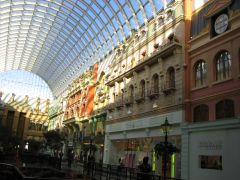
\includegraphics[width=.45\linewidth]{images/example_1}} \quad
        \subfloat[Pan ma signo.]
        {\label{fig:example-b}%
         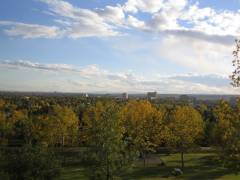
\includegraphics[width=.45\linewidth]{images/example_2}} \\
        \subfloat[Methodicamente o uno.]
        {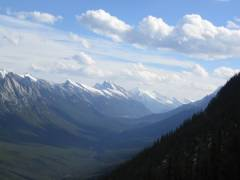
\includegraphics[width=.45\linewidth]{images/example_3}} \quad
        \subfloat[Titulo debitas.]
        {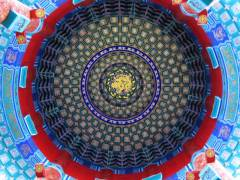
\includegraphics[width=.45\linewidth]{images/example_4}}
        \caption[Bilder.]{Beispielbilder von jMonkey.}\label{fig:example}
\end{figure}






